\chapter{Introduction}
%%%%%%%%%%%%%%%%%%%%%%%%%%%%%%%%%%%%%%%%%%%%%%%%%%%%%%%%%%%%%%%%%%%%%%%%%%%%%%%%%%%%%%%%%%%%%%%%%%%%%%%%%%%%%%%%%%%%%%%%%%%
\section{Contexte}
La \textbf{réalité virtuelle} est une simulation informatique interactive immersive, en temps réel. Elle peut être constituée d'une simulation visuelle, sonore ou haptique d'environnements réels ou imaginaires. Le but de la réalité virtuelle est de permettre à une personne d'effectuer une activité sensori-motrice et cognitive dans un monde créé numériquement. L'immersion est réalisée à l'aide de dispositifs tels que des casques (\textit{OcculusRift} par exemple), des gants connectés, etc. \\
La réalité virtuelle peut être utilisée pour les \textsf{Serious Games} (voir~\cite{SeriousGame}). Le \textsf{Serious Game} est un logiciel combinant une intention "sérieuse" avec les jeux par exemple dans un contexte pédagogique ou de rééducation. Il a pour but de rendre attrayants les jeux ludiques. Par exemple, les \textsf{Serious Games} peuvent être utilisés pour la santé (le site LudoMedic~\cite{LudoMedic} du studio CCCP~\cite{cccp}).\\

Le projet \textit{Virtual-Vertigo} est un \textsf{Serious Game} mis en place afin d'aider les personnes à combattre le \textbf{vertige} en utilisant la réalité virtuelle.\\
Ce trouble affecte une personne dans le contrôle de sa situation dans l'espace. Il peut survenir dans différentes circonstances ou causes à tout âge. Plusieurs symptômes définissent le vertige : 
\begin{itemize}
\item une illusion de mouvements,
\item une impression de désorientation et déséquilibre,
\item une crise de panique,
\item bien d'autres.
\end{itemize}
A noter que les symptômes sont différents pour chaque personne. \\
Le vertige peut entraîner une phobie : l'acrophobie (la peur du vide). Cette phobie est une peur extrême et irrationnelle des hauteur. Les acrophobes souffrent de peur panique lorsqu'ils sont en hauteurs et veulent à tout prix redescendre. \\

Selon les spécialistes, le vertige et l'acrophobie se soignent généralement avec une psychothérapie. Cependant, depuis quelques années, ils commencent à faire des thérapies utilisant la réalité virtuelle. Cette thérapie permet aux personnes d'affronter leurs peurs. A noter que cette thérapie n'a pas encore fait ses preuves. En effet les résultats sont partiels et incertains (pour plus d'informations voir \cite{acrophobie}).

%%%%%%%%%%%%%%%%%%%%%%%%%%%%%%%%%%%%%%%%%%%%%%%%%%%%%%%%%%%%%%%%%%%%%%%%%%%%%%%%%%%%%%%%%%%%%%%%%%%%%%%%%%%%%%%%%%%%%%%%%%%

\section{Projet Virutal-Vertigo}
\textit{Virtual-Vertigo} est un projet de développement \textit{Web mobile 3D}. Le but de ce projet est de réaliser un exercice permettant de combattre la peur du vide. En utilisant des casques de réalité virtuelle en carton contenant un \textsf{smartphone} et des lentilles, l'exercice se déroule dans une réalité virtuelle modélisant la vue d'une planche reliant deux immeubles. La personne effectuant la simulation doit traverser cette planche afin d'atteindre l'immeuble d'en face.\\

Dans ce projet, on emploie un dispositif de \textit{Google CardBoard} pour réaliser le casque de réalité virtuelle. Le monde virtuel 3D sera affiché via la \textit{technologie Web X3DOM} qui permet d'afficher des scènes 3D dans un navigateur. Un utilisateur s'immerge à travers ce dispositif dans le monde virtuel en se déplaçant sur une planche reliant deux immeubles. Un \textit{Kinect} sera utilisé pour récupérer les mouvements et les déplacements de la personne afin de les reporter dans le monde virtuel. Le \textit{Kinect} doit être connecté à un serveur pour transmettre les données capturées aux navigateurs sur \textsf{smartphone} et PC. En outre, des solutions pour rendre l'immersion de l'utilisateur dans le monde virtuel plus réaliste seront abordées.

\begin{figure}[H]
\centering
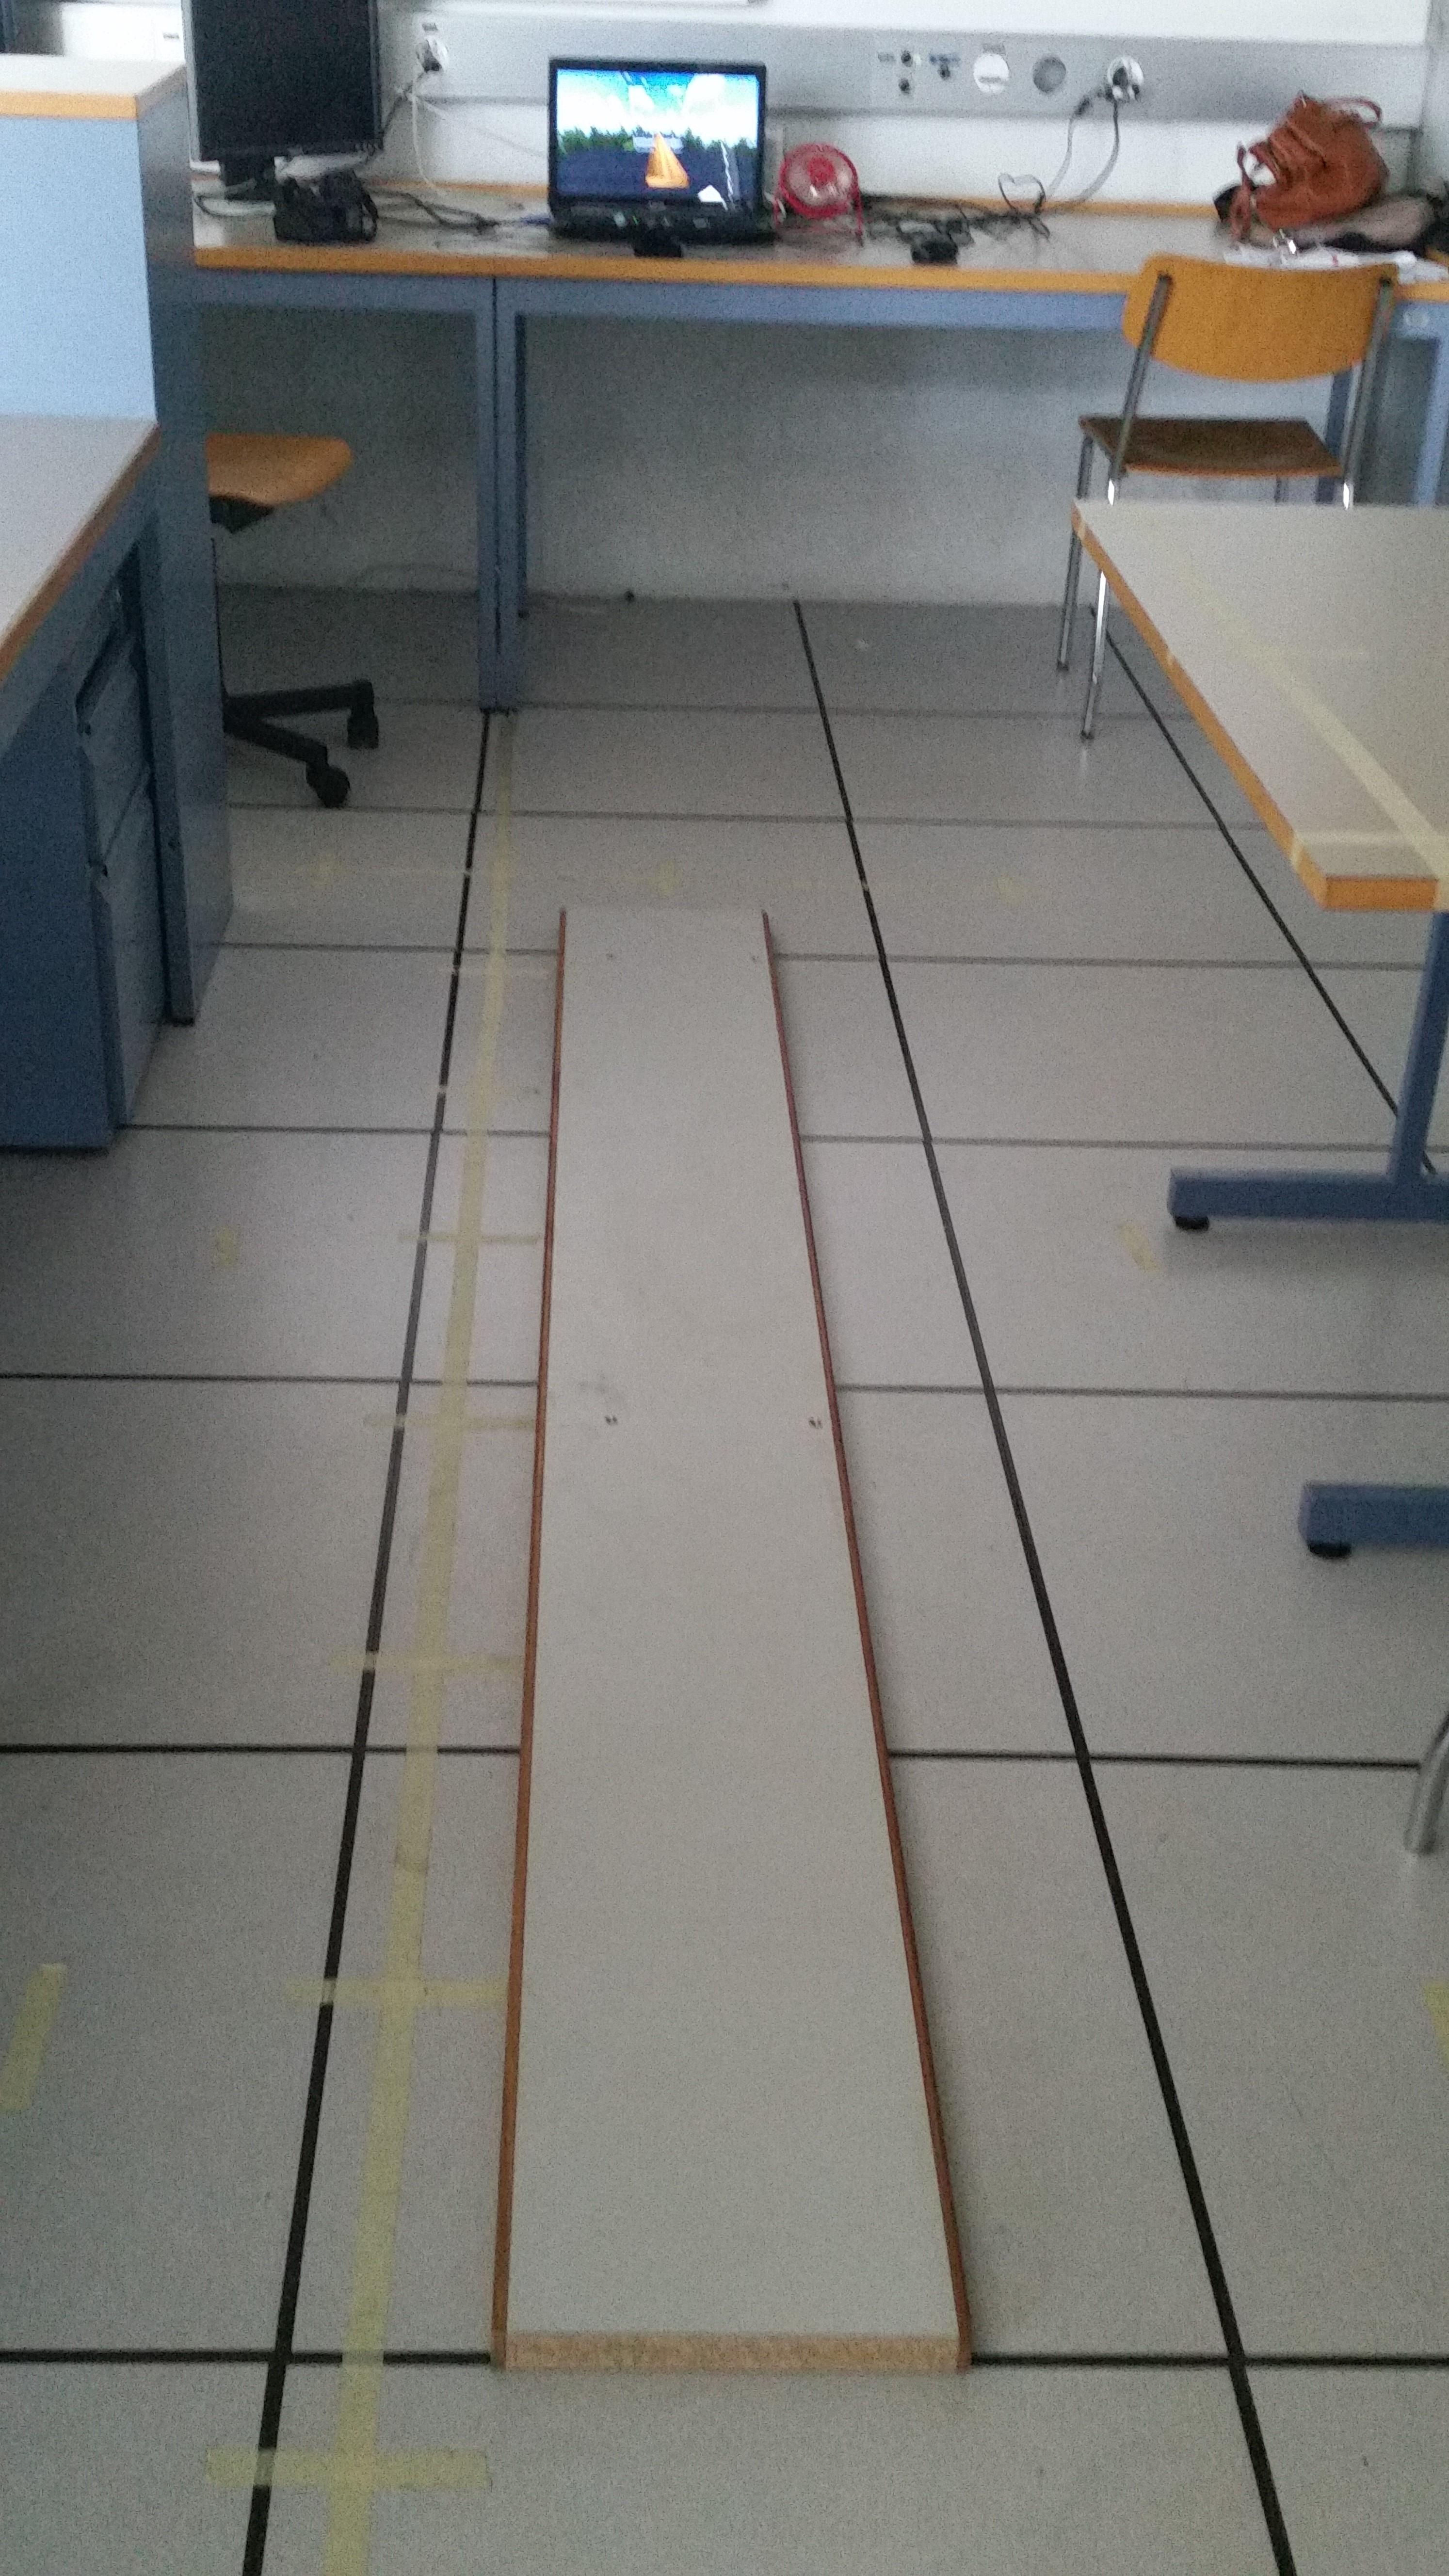
\includegraphics[scale=0.05]{vueReelle3.jpg}
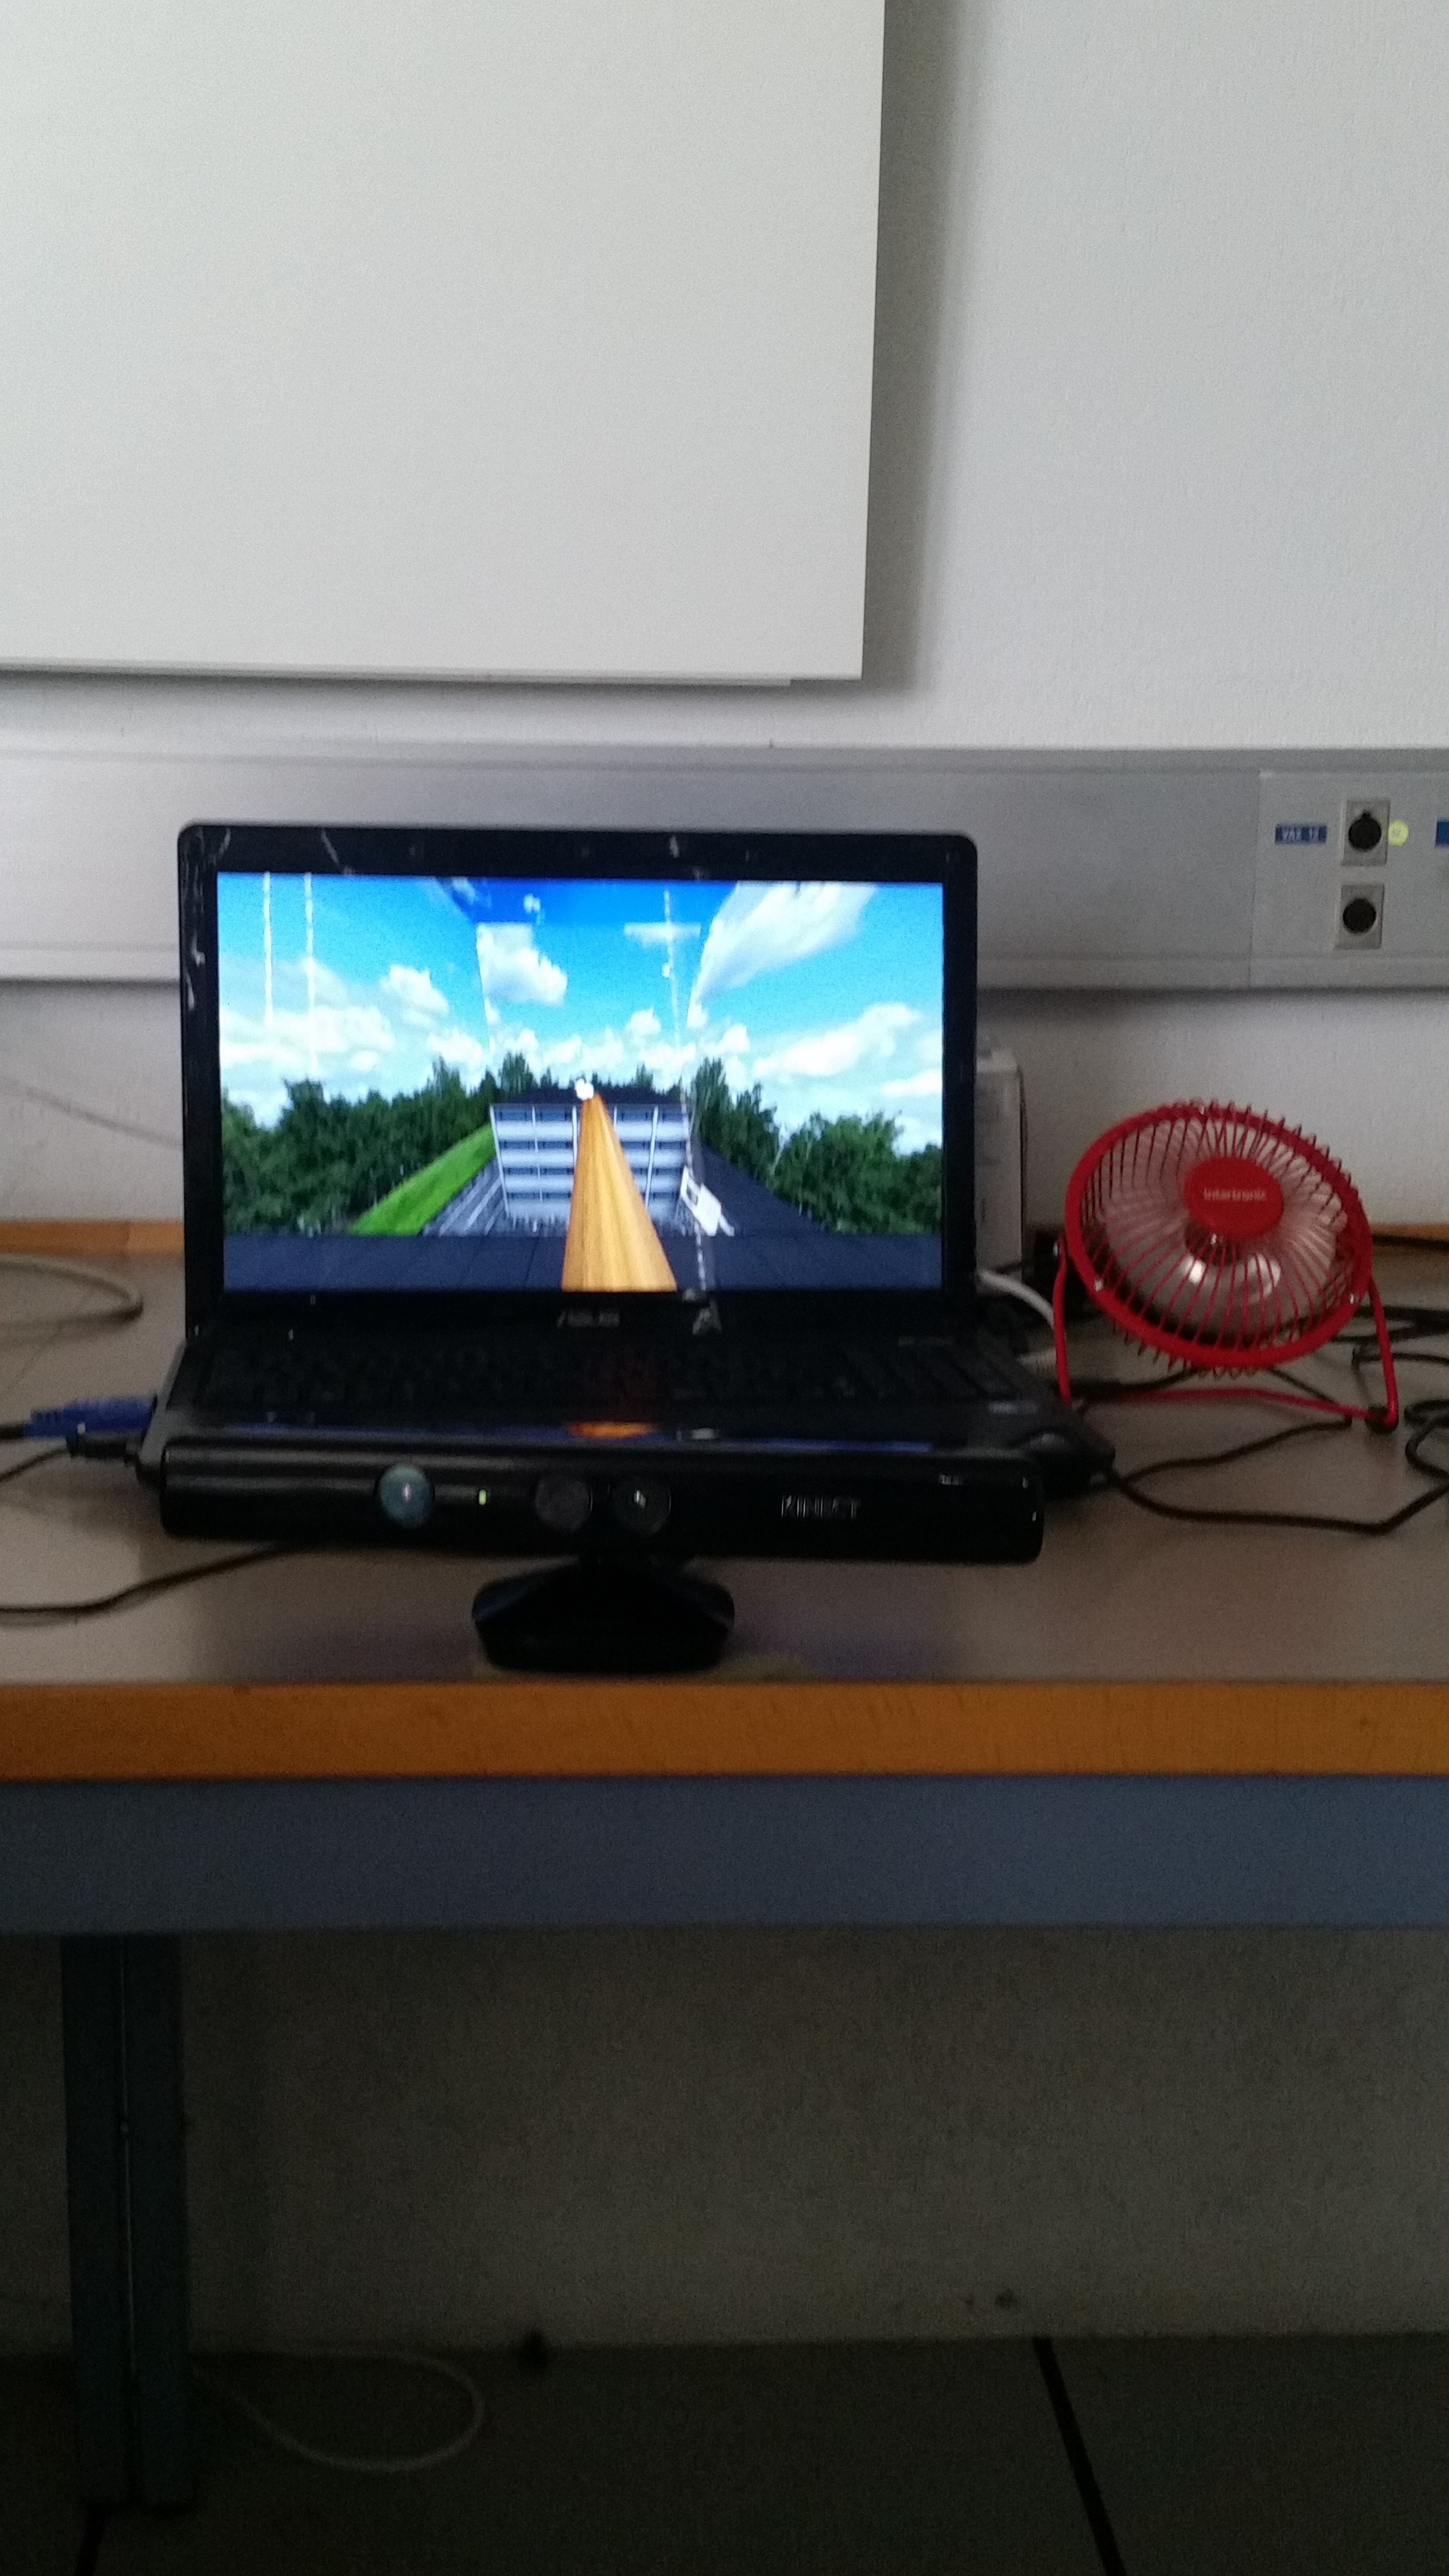
\includegraphics[scale=0.05]{vueReelle2.jpg}
\caption{\label{installation} Illustration de l'installation mise en place}
\end{figure}

La figure~\ref{installation} illustre l'installation mise en place pour le projet \textit{Virtual-Vertigo}.\\

A noter qu'un projet \textit{Ctrl Stress} développé par \textsc{M. Daniel Mestre}, psychologue et responsable du \textsf{Centre de Réalité Virtuelle de Méditerranée}, visant à vaincre la peur du vide avec la réalité virtuelle a déjà été mis en place a priori avec des \textit{Occulus Rift}. Pour lire un article sur ce projet, voir~\cite{cnrs}. Une étude~\cite{etude} a également été réalisée sur ce projet.\\
La principale différence entre \textit{Virtual-Vertigo} et \textit{Ctrl Stress} est que \textit{Virtual-Vertigo} permet à n'importe quelle personne possédant un \textit{Kinect} et des \textit{Google CardBoard} de l'utiliser alors que \textit{Ctrl Stress} n'est pas disponible. De plus le dispositif de \textit{Crtl Stress} est probablement cher.\\

A noter également qu'un glossaire décrivant toutes les technologies et les outils utilisés dans le projet \textit{Virtual-Vertigo} est disponible en annexe~\ref{glossaire}.

%%%%%%%%%%%%%%%%%%%%%%%%%%%%%%%%%%%%%%%%%%%%%%%%%%%%%%%%%%%%%%%%%%%%%%%%%%%%%%%%%%%%%%%%%%%%%%%%%%%%%%%%%%%%%%%%%%%%%%%%%%%

\section{Organisation du projet}
Le projet \textit{Virtual-Vertigo} dans son intégralité a été séparé en deux parties : 
\begin{enumerate}
\item Le \textsf{projet de semestre} était d'une durée équivalente à 3 semaines à temps complet, réparties sur un semestre. A la suite de ce travail, les bases du projet ont été mises en place :
\begin{itemize}
\item la construction des \textit{Google CardBoard},
\item la modélisation d'une vue basique 3D,
\item l'adaptation de la vue aux lunettes (stéréoscopie),
\item le choix entre les différentes technologies possibles pour l'échange et la capture des données,
\item la rotation d'un objet dans la vue 3D en fonction du smartphone,
\item le choix du \textit{Kinect} utilisé,
\item une rapide prise en main du \textit{Kinect}. \\

\end{itemize}

\item Lors du \textsf{travail de Bachelor} d'une durée de 12 semaines à temps complet, les éléments suivant ont été réalisés selon des plannings en annexe~\ref{plannings} :
\begin{itemize}
\item la modélisation de la vue finale (section~\ref{immeubles}~et~\ref{textures}),
\item le partage des données entre les outils (\textit{Kinect}, serveur et clients HTML) (section~\ref{serveur}~et~\ref{serveur2}),
\item la création du personnage virtuel (section~\ref{personnages}),
\item le déplacement de la personne dans la réalité virtuelle en fonction de la position de la tête (section~\ref{avancement}),
\item l'animation des membres de la personne dans la réalité virtuelle (section~\ref{animationPersonnage}),
\item l'adaptation de la vue sur le smartphone en fonction de la rotation de la tête (section~\ref{orientation}),
\item l'ajout de solutions pour une immersion plus réaliste (section~\ref{realisme}).
\end{itemize}

\end{enumerate}
